\section{Two-sample testing for SBMs}
\label{sec:ch8:twosamplesbm}

In Section \ref{sec:ch8:twosample}, we saw a situation where we had two networks which we thought could be effectively characterized with RDPG. Further, we knew that the communities were the same across both networks: that is, we knew that community $1$ in the first network was the same as community $1$ in the second network, so on and so forth all the way up to community $K$. In this situation, we found that we could test whether the latent positions for the underlying RDPGs are the same; that is, whether $H_0: X^{(1)} = X^{(2)}W$ against $H_A: H^{(1)} \neq X^{(2)}W$. We called this the two-sample hypothesis test for RDPGs. 

What if we can take this a step further, however, and we can say that the networks are realizations of SBMs? How can we check whether the block matrices are the same? If you remember from Section \ref{sec:ch5:psd_block:lpm_fromsbm}, we learned that the latent position matrix for positive semi-definite block matrices is just a function of the community assignment vector and the block matrix. Therefore, if two networks have the same community assignment vectors but their positive semi-definite block matrices are unequal, their latent position matrices are unequal. Therefore, we could use the machinery that we developed in Section \ref{sec:ch8:twosample} to test whether the block matrices are unequal.

However, we can approach this question more directly for SBMs: we can test whether the block matrices are unequal directly. In Case Study \ref{box:ch8:twosampsbm:ex}, we develop an example we will work with for this section.

\begin{floatingbox}[h]\caption{Case Study: Traffic patterns}
We have two networks which summarize the traffic patterns between $n=100$ towns (represented by the nodes in our network) across $K=3$ states (represented by the communities in our network). The first 45 towns are in New York (NY, the first community), the second 30 towns are in New Jersey (NJ, the second community), and the third 25 towns are in Pennsylvania (PA, the third community). Our goal is to examine traffic pattern differences during the daytime compared to night time.

For a month, we measure the number of drivers who commute from one town to the other in a specified time window, and if more than $1,000$ drivers regularly make this commute, we add an edge between the pair of towns. In general, we know that people tend to commute more frequently within their state, so the probabilities that an edge exists between a pair of towns in the same state exceeds the probabilities that an edge exists between a pair of towns which are not in the same state. Now, here's the twist: we have measured the first network between 7 AM and 7 PM (covering the bulk of the work day), and the second network between 7 PM and 7 AM (covering the bulk of night time). We know that a lot of people in New Jersey tend to commute to new York for the work day, so we the probability of an edge existing between a New Jersey town and a New York town are higher during the day than the night.

We don't think that driving patterns themselves really change too much otherwise, but we do think that the probability of an edge existing is about $50\%$ higher during the daytime for all pairs of communities in the network.
\end{floatingbox}

Let's generate the community assignment vector and the block matrices for the day and night time. The day time network will be network $(1)$, and the night time network will be network $(2)$:
\begin{lstlisting}[style=python]
import numpy as np
from graspologic.simulations import sbm
ns = [45, 30, 25]  # number of students

# z is a column vector indicating which state each
# town is in
z = np.array(["NY" for i in range(0, ns[0])] + 
              ["NJ" for i in range(0, ns[1])] +
              ["PA" for i in range(0, ns[2])] )

Bnight = np.array([[.3, .15, .15], [.15, .3, .15], [.15, .15, .3]])
Bday = Bnight*1.5  # day time block matarix is 50% more than night

# people tend to commute from New Jersey to New York during the day
Bday[0, 1] = .4; Bday[1,0] = .4

Anight = sbm(ns, Bnight)
Aday = sbm(ns, Bday)
\end{lstlisting}

The block matrices, and the two network samples, are shown in Figure \ref{fig:ch8:twosampsbm:ex}.

\begin{figure}
    \centering
    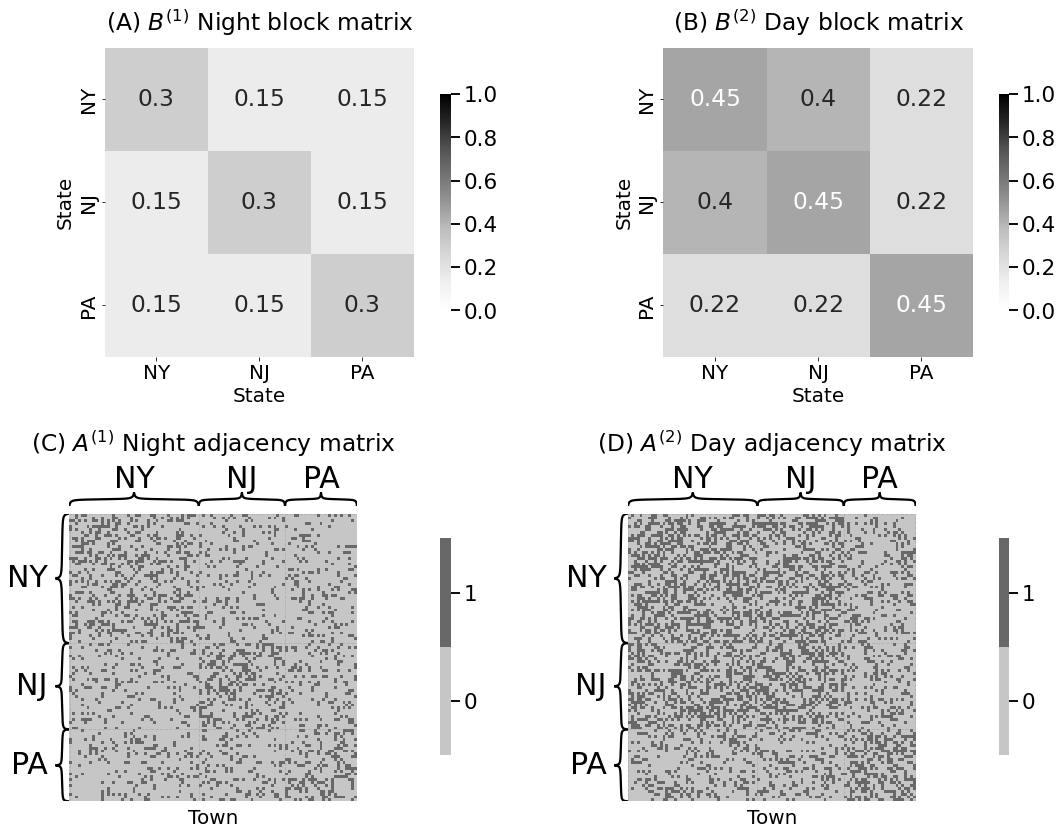
\includegraphics[width=\linewidth]{applications/ch8/Images/twosamp_sbm_ex.png}
    \caption[Two-sample SBM comparison]{\textbf{(A)} the block matrix for night time, \textbf{(B)} the block matrix for day time, \textbf{(C)} the adjacency matrix for night time, \textbf{(D)} the adjacency matrix for day time.}
    \label{fig:ch8:twosampsbm:ex}
\end{figure}

\subsection{Testing whether the block matrices in an SBM are different}

Based on what we learned above, we know ahead of time that the block matrices for the SBMs are different. However, how can we actually test this? Well, let's start by being clear about what we mean by "different". To make this a little big more mathemattical, we'll introduce some new variables for the block matrices during the day time ($B^{(1)}$) and at night time ($B^{(2)}$) clearly. The block matrices are:

\begin{align*}
    B^{(1)} &= \begin{bmatrix}
    b^{(1)}_{11} & b^{(1)}_{12} & b^{(1)}_{13} \\
    b^{(1)}_{21} & b^{(1)}_{22} & b^{(1)}_{23} \\
    b^{(1)}_{31} & b^{(1)}_{32} & b^{(1)}_{33}
    \end{bmatrix}; \;\;\; B^{(2)} = \begin{bmatrix}
    b^{(2)}_{11} & b^{(2)}_{12} & b^{(2)}_{13} \\
    b^{(2)}_{21} & b^{(2)}_{22} & b^{(2)}_{23} \\
    b^{(2)}_{31} & b^{(2)}_{32} & b^{(2)}_{33}
    \end{bmatrix}
\end{align*}
The hypothesis we want to test is the null hypothesis that the block matrices are the same, $H_0: B^{(1)} = B^{(2)}$, against the alternative hypothesis that the block matrices are different, $H_A: B^{(1)} \neq B^{(2)}$. For a matrix, remember that two matrices are equal if all of the entries are identical, and two matrices are unequal if at least one of the entries are unequal. We can reformulate the null and alternative hypotheses with this logic.

For the null hypothesis, $H_0: B^{(1)} = B^{(2)}$, the statement is therefore equivalent to saying that for all pairs of communities $k$ and $l$, $b^{(1)}_{kl} = b^{(2)}_{kl}$. We will write each of these statements down as individual hypotheses for all pairs of communities, using the convention $H_{0, kl}: b_{kl}^{(1)} = b^{(2)}_{kl}$. 

The null hypothesis $H_0$ is therefore equivalent to saying that for every pair of communities $k$ and $l$, $H_{0,kl}$ is true. 

For the alternative hypothesis, $H_A: B^{(1)} \neq B^{(2)}$, the statement is therefore equivalent to saying that for at least one pair of communities $k$ and $l$, $b^{(1)}_{kl} \neq b^{(2)}_{kl}$. We will write down each of these statements as well as individual hypotheses for all pairs of communities, using the convention $H_{A, kl} : b_{kl}^{(1)} \neq b^{(2)}_{kl}$. The alternative hypothesis $H_A$ is therefore equivalent to saying that for at least one pair of communities $k$ and $l$, that $H_{A,kl}$ is true.

Now that we have broken a statement about two matrices down into numerous statements about two probabilities, we have almost completed our job. As it turns out, we have already seen the way we will test this, back in testing for differences in Section \ref{sec:ch7:testing}. Seeking to test whether a pair of block probabilities between communities $k$ and $l$ are the same, $H_{0,kl}$, against whether the pair of block probabilities between communities $k$ and $l$ are different, $H_{A, kl}$, is the two-sample testing problem, like Section \ref{sec:ch7:testing:twosample}. We addressed this problem before using Fisher's exact test, and that is what we will do here, too.

Remember that with Fisher's exact test, for two probabilities that we want to compare, we construct a contingency table. In this case, we will have $\binom K 2 + K$ contingency tables (one for each unique pair of communities, plus the on-diagonal edges where both nodes have the same community), which are shown in Table \ref{tab:ch8:twosampl_sbm:cont}.

\begin{table}[h]
    \centering
    \begin{tabular}{c|c| c}
         & $(1)$, night time & $(2)$, day time  \\
         Number of edges & $a$ & $b$ \\
         Number of non-edges &$c$ & $d$
    \end{tabular}
    \caption[Two-sample SBM contingency table.]{An example of a contingency table for testing for a difference in the block matrices between two SBMs. $\binom K 2$ of these contingency tables are constructed, corresponding to the contingency tables between nodes in community $k$ and $l$ for all possible pairs of communities.}
    \label{tab:ch8:twosampl_sbm:cont}
\end{table}

In the table, entry $a$ is the total number of edges between nodes of community $k$ with nodes of community $l$ in the daytime network, and $b$ is the total number of edges between nodes of community $k$ with nodes of community $l$ in the daytime network. The entry $c$ the total number of potential edges between nodes of community $k$ with nodes of community $l$ in the day time network that do not exist (the number of adjacencies with an adjacency of zero), and the entry $d$ is the total number of potential edges between nodes of community $k$ with nodes of community $l$ in the night time network that do not exist. 

We implement this using \texttt{numpy} and \texttt{scipy}, just like we did before, but this time for each pair of communities. To identify which adjacency matrix entries correspond to a given pair of communities, we use \texttt{np.outer}. Since the network is simple, we also exclude the on-diagonal entries, and avoid double counting by only looking at the upper-right triangle of the adjacency matrix:

\begin{lstlisting}[style=python]
from scipy.stats import fisher_exact

K = 3
Pvals = np.empty((K, K))
# fill matrix with NaNs
Pvals[:] = np.nan

# get the indices of the upper triangle of Aday
upper_tri_idx = np.triu_indices(Aday.shape[0], k=1)
# create a boolean array that is nxn
upper_tri_mask = np.zeros(Aday.shape, dtype=bool)
# set indices which correspond to the upper triangle to True
upper_tri_mask[upper_tri_idx] = True

for k in range(0, K):
    for l in range(k, K):
        comm_mask = np.outer(z == (k+1), z == (l + 1))
        table = [[Aday[comm_mask & upper_tri_mask].sum(), Anight[comm_mask & upper_tri_mask].sum()],
                 [(Aday[comm_mask & upper_tri_mask] == 0).sum(), (Anight[comm_mask & upper_tri_mask] == 0).sum()]]
        Pvals[k,l] = fisher_exact(table)[1]
\end{lstlisting}

This gives us a matrix of $p$-values, whose $p$-values correspond to tests of $H_{0, kl}$ against $H_{A, kl}$ for all pairs of communities $k$ and $l$. However, this still does not give us an answer to our original question, whether the block matrices $B^{(1)}$ and $B^{(2)}$ were the same against the alternative that the block matrices $B^{(1)}$ and $B^{(2)}$ were different.

\subsubsection*{Adjusting for multiple comparisons}

When performing multiple statistical tests, we run into the multiple hypothesis correction problem. Let’s imagine that we have $5000$ coins, and each of these coins has a true probability of landing on heads of $0.5$. We flip each coin 
$500$ times, and for each coin $i$, we estimate the probability that the coin lands on heads by just counting the number of heads and dividing by $500$. For each coin, we want to test whether the probability that the coin lands on heads is different from $0.5$. In symbols, we want to test $H_0^{(i)} : p^{(i)} = 0.5$ against $H_A^{(i)}: p^{(i)} \neq 0.5$. For this problem, an appropriate statistical test is known as the Binomial test, which is described in Appendix \ref{app:ch14:hypotest_intro}. For the purposes of this section, all that you need to know is that it is a way of testing whether the data supports (or does not support) that a probability is equal to a fixed constant. Let's run our experiments:

\begin{lstlisting}[style=python]
import numpy as np
from graspologic.simulations import er_np
import seaborn as sns
from scipy.stats import binom_test

ncoins = 5000 # the number of networks
p = 0.5  # the true probability
n = 500  # the number of flips

# the number of heads from each experiment
experiments = np.random.binomial(n, p, size=ncoins)

# perform binomial test to see if the number of heads we obtain supports that the
# true probabiily is 0.5
pvals = [binom_test(nheads_i, n, p=p) for nheads_i in experiments]
\end{lstlisting}


\begin{figure}
    \centering
    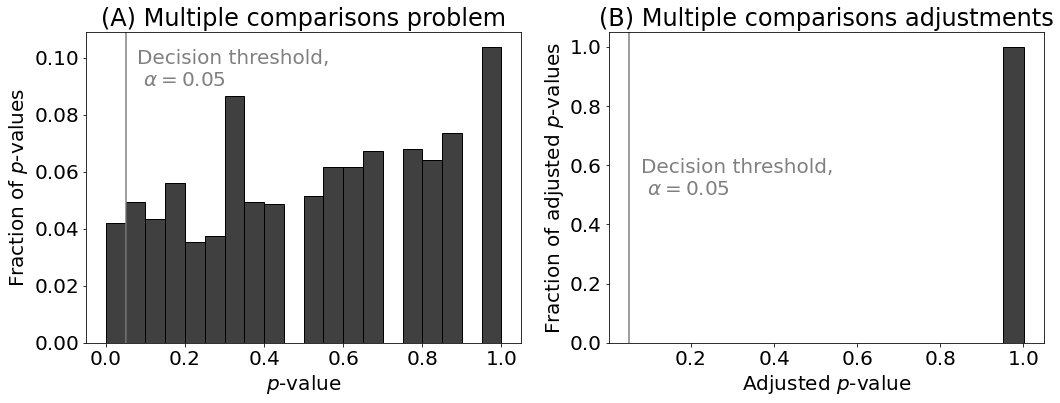
\includegraphics[width=\linewidth]{applications/ch8/Images/twosampsbm_mc.png}
    \caption{\textbf{(A)} a histogram of the $p$-values before multiple comparisons adjustment, \textbf{(B)} a histogram of the $p$-values after adjusting for multiple comparisons, by preserving the FWER via Holm-Bonferroni correction.}
    \label{fig:ch8:twosampsbm:mc}
\end{figure}
A histogram of the $p$-values from all $5000$ tests (one for each coin) are shown in Figure \ref{fig:ch8:twosampsbm:mc}(A). In general, we will correctly reject the alternative hypothesis, and accept the null hypothesis. This is great, since $p_i$ is, in fact, $0.5$ as specified by the null hypothesis $H_{0}^{(i)}$. However, we notice something particularly strange: For a portion of the tests, we are, in-fact, wrong. We obtain many $p$-values which are under our decision threshold of $\alpha = 0.05$, and would incorrectly report that the alternative hypothesis is correct, and $p_i$ is not $0.5$. This is wrong, and extremely problematic! Remember that the $p$-value was defined as the probability that the null hypothesis (here, that $p_i = 0.5$) would be incorrectly rejected in favor of the alternative hypothesis (here, that $p_i \neq 0.5$). In fact, if the null hypothesis were true, we would expect to see $p$-values of at most $\alpha$ being reported about $\alpha$ of the time (this assumes all of the coins are independent, but even when they are not all independent, we still obtain a similarly shocking conclusion). This means that with $n=5000$ tests and $\alpha = 0.05$, we would expect to be wrong about $n\cdot \alpha = 50$ times.

Basically, the problem here is that while each test individually only has a $\alpha = 0.05$ chance of incorrectly rejecting the null hypothesis (when it is true), by running multiple tests, we have increased the familywise error rate to be well north of $\alpha = 0.05$. The \textit{familywise error rate} (FWER) is the probability that we made an error and incorrectly rejected the null hypothesis for any one of the hypothesis tests we ran. You can read more about this problem here \cite{Ryan1959Jan}.

As practicians, it feels like it would be pretty problematic to report an analysis and know that an arbitrary fraction of your conclusions are wrong just by random chance. For this reason, a focus of statistics in recent decades has been the development of methods which, in effect, inflate the $p$-values based on the number of tests that we perform, so that we run into this issue at much lower rate than $\alpha$ of the time. These strategies are collectively known as \textit{multiple comparisons adjustments}. We won't go into too many details with how multiple comparisons adjustments are performed, but in general given a list of $p$-values \texttt{pvals}, you can adjust the $p$-values using the \texttt{multipletests()} method from \texttt{statsmodels}. This will give you protection for this ``multiple comparisons'' issue in your analyses, and make you a more conservative statistician. Like in Section \ref{sec:ch8:twosample:lpt_vs_ldt}, conservative statistical approaches are approaches which tend to err on the side of caution.

Let's see what happens when we adjust our $p$-values here using a popular method called Bonferroni-Holm adjustment \cite{Holm1979}:
\begin{lstlisting}[style=python]
from statsmodels.stats.multitest import multipletests

alpha = 0.05  # the desired alpha of the test
_, adj_pvals, _, _ = multipletests(pvals, alpha=alpha, method="holm")
\end{lstlisting}

A histogram of the $p$-values after adjustment is shown in Figure \ref{fig:ch8:twosampsbm:mc}(B). After adjusting for multiple comparisons, we end up with all of the $p$-values being $1$. Therefore, we never incorrectly reject the null hypothesis anymore.

In general, for multiple hypothesis correction, we recommend using Holm-Bonferroni correction, which is encoded with the parameter \texttt{method="holm"}. We recommend the use of the Holm-Bonferroni approach because it ensures that our $p$-value produced by using multiple statistical tests controls the FWER with no requirements as to the problem we glossed over previously, the dependence of the hypotheses being tested. This may give us adjusted $p$-values that are a little higher than several other methods (such as the popular Benjamini-Hochberg procedure), but in general we prefer to err on the side of caution when reporting scientific discoveries and do not want to spend effort investigating hypothetical dependencies amongst our hypothesis tests.

Let's adjust the $p$-values that we estimated for the pairwise community comparisons for our networks, upper-right symmetrize the resulting matrix of $p$-values (because we only ran tests on the upper-right triangle of the adjacency matrix), and then plot the result:
\begin{lstlisting}[style=python]
from graspologic.utils import symmetrize

Pvals_adj = multipletests(Pvals.flatten(), method="holm")[1].reshape(K, K)
Pvals_adj = symmetrize(Pvals_adj, method="triu")
\end{lstlisting}

\begin{figure}
    \centering
    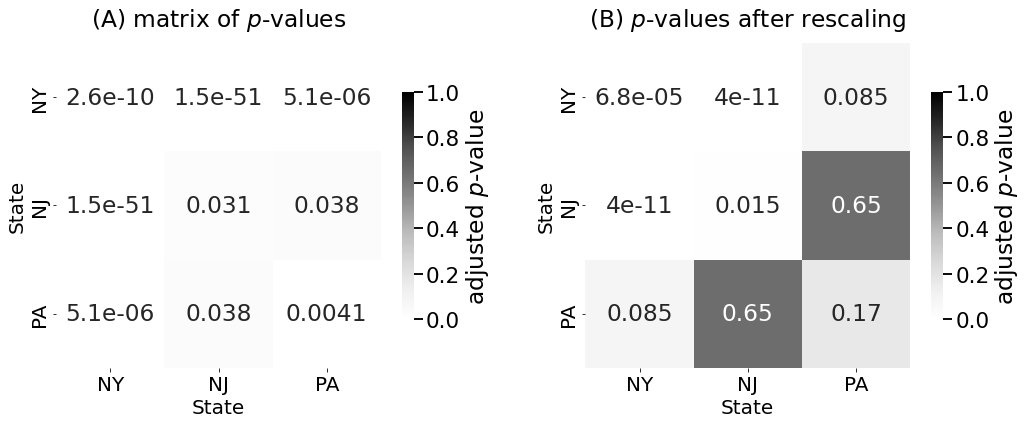
\includegraphics[width=\linewidth]{applications/ch8/Images/twosamp_sbm_pvals.png}
    \caption[$p$-values for differences between block matrices]{\textbf{(A)} $p$-values for test of a difference between the block matrices, \textbf{(B)} $p$-values for test of a difference between the block matrices, after rescaling.}
    \label{fig:ch8:twosampsbm:pval_mtx}
\end{figure}

The matrix of $p$-values (after adjustment for multiple comparisons) is shown in Figure \ref{fig:ch8:twosampsbm:pval_mtx}(A). The $p$-values are all extremely small, so we can conclude that the block matrices $B^{(1)}$ and $B^{(2)}$ differ for all entries. The $p$-value for the test of $H_0$ that the block matrices are identical against $H_A$ that the block matrices are different can be taken to be the minimum of all of the adjusted $p$-values:

\begin{lstlisting}[style=python]
pval_dif = Pvals_adj.min()
print("p-value of block matrix difference: {:.4f}".format(pval_dif))
# p-value of block matrix difference: 0.0000
\end{lstlisting}
which is so small that it rounds to $0$. With $\alpha = 0.05$ as usual, we reject the null hypothesis that the block matrices are identical in favor of the alternative that the block matrices are different. 

\subsection{Testing whether the block matrices in an SBM are multiples of one another}

Back in Section \ref{sec:ch5:prop:rndeg} we learned about a useful summary statistic for random networks, known as the expected density. The expected network density could be written as:
\begin{align*}
\mathbb E[density(\mathbf A)] &= \frac{\sum_{i = 1}^n \mathbb E[\mathbf d_i]}{n(n - 1)} 
\end{align*}
Which could be thought of as the expected average degree of each node in the network, divided by the maximum possible degree each node could have. 

As it turns out, the network density plays an extremely large role in virtually every property of networks which we estimate in machine learning, including the block matrices. Remember from Concept \ref{box:ch5:dcsbm:exp_deg}, that for a $SBM_n(\vec z, B)$ random network, the average degree for a node in community $k$ was:
\begin{align*}
    \mathbb E[\mathbf d_i ; z_i = k] &= \sum_{l \neq k} n_l b_{lk} + (n_k - 1)b_{kk}
\end{align*}
so it is clear that the expected node degree is a function of the block matrix. As the expected density is a function of the expected degrees, the expected density is a function of the block matrix, too. We could also reverse this argument, and establish a relationship between the block matrices and the expected density in the network.

This means that if the expected densities are different, the block matrices will, by default, also be different.

For instance, in our example, we know that the probability of an edge existing between two cities is, in general, about $50\%$ higher during the daytime compared to the night time. We don't want to have our answer just be a product of the fact that there were just more edges in the daytime network. Rather, we want to find the topological difference between the two networks; that is, that the day time driving patterns between New Jersey and New York towns went above and beyond the $50\%$ increase we otherwise saw. For this reason, we revamp our hypothesis a little bit.

If you remember, our hypothesis that we ran above was the null hypothesis $H_0: B^{(1)} = B^{(2)}$ that the two block matrices are the same against the alternative $H_A: B^{(1)} \neq B^{(2)}$ that the block matrices differ. We will change this up a little bit. Now, our null hypothesis becomes $H_0: B^{(1)} = \alpha\cdot B^{(2)}$ that the two block matrices are the same up to a rescaling against $H_A: B^{(2)} \neq \alpha\cdot B^{(2)}$, that they differ even after possible rescalings. How do we interpret this?

In this case, the value $\alpha$ is chosen to be the difference in the expected network densities between the day time and night time networks, the quantity $\alpha = \frac{p^{(1)}}{p^{(2)}}$. In practice, what we use is an estimate of this quantity, $\hat \alpha = \frac{\hat p^{(1)}}{\hat p^{(2)}}$, where $\hat p^{(1)}$ is the network density of the night time network and $\hat p^{(2)}$ is the network density of the day time network. Accepting the alternative hypothesis here means that the block matrices of the day and night time network are not simply multiples of each other.

\begin{floatingbox}[h]\caption{Case Study: Bilateral symmetry in fruit fly brains}
\label{box:ch8:twosamp_sbm:conn}
It is fairly well-established that the brain of human beings is asymmetric: different sides of your brain are responsible for related, but distinct, functions \cite{Springer2001Sep}. This was definitively established in the 1860s by a scientist named Paul Broca, who discovered that patients with brain lesions to the same area of the left frontal portion of the brain experienced similar symptoms of speech loss. That two patients with similar lesions experienced the same symptoms provided evidence that brain function was \textit{localized}, in that different areas of the brain were responsible for different functions. Related observations made by psychologists led to conclusions that took this a step further, that different hemispheres of the brain were responsible for different functions.

In a recent paper \cite{Pedigo2022Nov}, investigators were able to connect a similar ``localization of connectivity'' in the wiring of the brain itself. The investigators used connectomes of a fruit fly for the left and right hemispheres, where the nodes were individual neurons and the edges were individual connections (called \textit{synapses}) between these neurons. Using the methods that we explained above, they were able to show that some types of cells in the brain had totally different densities of edges between the two hemispheres. After accounting for these hemisphere density disparities, several different cell types had similar connectivity patterns.
\end{floatingbox}

We address this problem very similarly to above, instead using the chi-squared test for non-unity probability ratios from \cite{Dunnett1977Dec, Chan2003Jan, Miettinen1985Apr}. We covered the chi-squared test in Section \ref{sec:ch7:modelselect} when we were covering model selection. We implement this using the bilateral connectome package \cite{neurodata2023Feb}, again showing the $p$-value matrix to visualize which combinations of communities are substantially different. This approach is described in \cite{Pedigo2022Nov}:

\begin{lstlisting}[style=python]
from pkg.stats import stochastic_block_test, combine_pvalues

stat, _, misc = stochastic_block_test(Anight, Aday,
    labels1=z, labels2=z, density_adjustment=True)
Pval_adj_rescaled = np.array(misc["corrected_pvalues"])
\end{lstlisting}

This new matrix of $p$-values is shown in Figure \ref{fig:ch8:twosampsbm:pval_mtx}(B), This shows that after we adjust the block matrix for changes in network density, the difference in the block probability for traveling between New York and New Jersey is still significant. This means that the density-adjusted block matrices are different, since the minimum corrected $p$-value is less than $0.05$.


The interpretation here is that, after adjusting for density, we can still reject the null hypothesis in favor of the alternative that the block matrices for day and night time are different, and that this difference can be accounted for by different traffic patterns between New York and New Jersey in day time versus night time. For an example of the use of these strategies in practice, check out Case Study \ref{box:ch8:twosamp_sbm:conn}.


\newpage

